\section{Object-based tiling scheme}

In this section we first introduce our object detection method. Based on this object detection, we describe our object-based tiling scheme and make comparison with state-of-art grid-like tiling schemes.

\subsection{Object Detection based on Quality-Bitrate Efficiency}

In the field of computer vision, there are many object detection algorithms which can cut a video into different content objects. However, in our video tiling scheme, the purpose of object  detection is little different. Actually we do not care if two adjacent tiles contain exactly the same object semantically. The most important thing is the probability of them to be allocated the same bitrate level by client. Even though two adjacent objects are different, if they have similar properties (like luminance, contrast, Depth of Field), we can also contain them in one tile because there is high probability for user to allocate them the same bitrate level.

To meet our purpose, for any rectangular tile which can be independently encoded, we define its \textbf{Quality-Bitrate Efficiency (QBE)} as follow:

\begin{alignat}{2}\
QBE = \frac{PSPNR_{highest} - PSPNR_{lowest}}{B_{highest} - B_{lowest}} \label{QBE}
\end{alignat}

where $PSPNR_{highest}$ / $PSPNR_{lowest}$ denotes the PSPNR value of this tile's highest / lowest bitrate version, and $B_{highest}$ / $B_{lowest}$ denotes the bitrate of this tile's highest / lowest bitrate version. In order to eliminate the influence for PSPNR by different user viewpoint positions, we only consider luminance, texture complexity and Depth-of-Field in QBE computation. These informations can be obtained completely on server-side.

In a video frame, different objects have different QBE. QBE is highly related to properties of content objects. According to PSPNR computation (Section 4), objects with very dark / light object luminance, complex texture or high depth of field, usually has higher QBE.

In perceived quality optimization, it is obvious that objects with high QBE is more likely to be allocated high bitrate (because it can improve more PSPNR in the same bandwidth cost), and objects with low QBE is more likely to be allocated low bitrate. So when two adjacent objects have similar QBE, they have high probability to be allocated the same bitrate level. 

\subsection{Tiling video by objects}

Based on above insights, we aim to cut the video into $T$ rectangular tiles of unequal size, such that content items within the same tile have similar QBE.

In this paper, tiling video by objects consists of 3 steps:

\textbf{Step 1: Partitioning the original video into 12*24 rectangular basic units of equal size.} 

Basic unit is the smallest unit of proposed object-based tiling. In the tiling process, each tile must be composed by one or several entire basic units which form a rectangular shape.

\textbf{Step 2: Computing QBE of each basic unit.}

We get QBE of each basic unit according to (\ref{QBE}). After that, suppose a tile $t$ consists of $N_t$ basic units $u_1$, $u_2$, ... , $u_{N_t}$ , we can compute its QBE Variance ($QBEV_t$) as follow:

\begin{alignat}{2}\
QBEV_t = \frac{\sum_{1 \le i \le N_{t}}{(QBE_{u_i} - E(QBE_{u_{i}}))^2}}{N_t}
\end{alignat}

where $E(QBE{u_i})$ is the average QBE of basic units in tile $t$:

\begin{alignat}{2}\
E(QBE_{u_i}) = \frac{\sum_{1 \le i \le N_{t}}{QBE_{u_i}}}{N_t}
\end{alignat}

A tile with high QBEV means visual properties (e.g. luminance, texture complexity) of objects in this tile have very different properties. A tile with low QBEV means objects in this tile are similar. So a good tiling scheme should keep each tile's QBEV value as low as possible.

\textbf{Step 3: Merging all basic units into T rectangular tiles, such that their weighted average QBEV is minimal.}

Suppose $V$ is the whole video frame. $R_i$ is the $i$th rectangular tile and $S_i$ is its area.This optimization problem can be formalized as following:

\begin{equation}
\begin{aligned}
\min \sum_{i = 1}^T QBEV_{i} S_i \hspace{3cm} \\
\text{s.t.} \bigcup _{i=1}^N R_{i} = V\hspace{3cm} \\
R_i \bigcap R_j = \emptyset \hspace{1cm} \forall 1 \le i, j \le T
\end{aligned}
\end{equation}

However, this optimization problem is a NP-hard problem, so we can not get the optimal solution in polynomial time. In practice, we apply a dynamic programming algorithm to get the suboptimal solution for this problem. In our implementation, we set $T = 72$ since it performs well in most situations.

\subsection{Comparison of object-based tiling and grid-like tiling}

We evaluate our tiling scheme and make comparison with traditional grid-like tiling schemes.

Fig. \ref{tiling} shows the PSPNR-bandwidth tradeoff of 3*6 grid tiling, 6*12 grid tiling, 12*24 grid tiling and proposed object-based tiling. 

  \begin{figure}
  \centering
  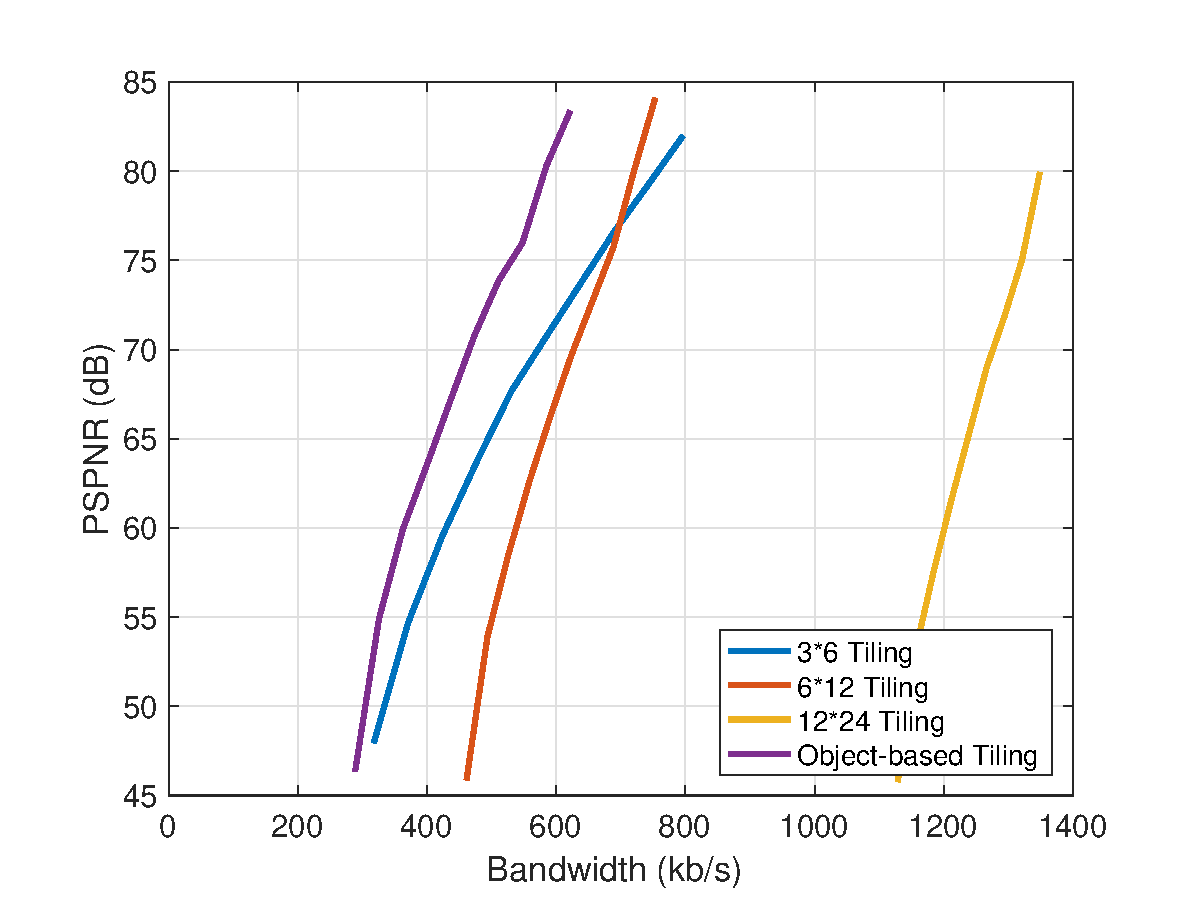
\includegraphics[width=2.5in]{images/tiling.eps}
  \caption{The PSPNR-bandwidth tradeoff of proposed Object-based Tiling scheme and traditional grid-like tiling scheme (3*6, 6*12 and 12*24).}
  \label{tiling}
  \end{figure}

For traditional gird-like tiling schemes, the performance of different tiling granularity depends on bandwidth. In low bandwidth, most part of video is allocated the lowest bitrate level. So there is no need to cut the video into many tiles. 3*6 tiling performs well because of its high bitrate efficiency. However, in high bandwidth, a coarse tiling granularity causes suboptimal bitrate allocation, so it is beaten by 6*12 tiling. Unfortunately, 12*24 tiling performs poorly in all bandwidth because of its serious bitrate efficiency problem.

Proposed object-based tiling scheme beats traditional grid-like tiling scheme of all bandwidth. In high bandwidth situation, it saves 20\% bandwidth compared with 6*12 grid-like tiling. Although 3*6 tiling's low bandwidth performance is near to proposed object-based tiling, its high bandwidth performance is far away from object-based tiling.
